\documentclass[a4paper]{book}


\usepackage[student]{Lecture}
%\lhead{Cours n°1 : Lithium au sein du tableau périodique}
\lhead{\leftmark} \chead{} \rhead{4.13}
\lfoot{IUT d'Orsay - BUT 2 MAT - 2024-2025} \cfoot{
\includegraphics[height=0.5cm]{cc-by-nc-sa.png}}  \rfoot{Jean-François Olivieri \quad \thepage}

\begin{document}

\begin{comment}
\begin{titlepage}
  \begin{sffamily}
  \begin{center}

    % Upper part of the page. The '~' is needed because \\
    % only works if a paragraph has started.
    \includegraphics[height=4cm]{logo.png}~\\[0.5cm]

    \textsc{\LARGE Université Paris-Saclay}\\[0.5cm]
    
    \textsc{\Large IUT d'Orsay - Département de Chimie}\\[0.5cm]
    
    \textsc{\large BUT 2, module 3.06 - Propriété des matériaux}\\[3.0cm]

    % Title
    \HRule \\[0.4cm]
    { \huge \bfseries Matériaux pour l'énergie\\[0.4cm] }

    \HRule \\[0.4cm]
    
       
    \textsc{\Large  Une introduction aux batteries}\\[0.5cm] 
    
    \textsc{\Large  Année 2023-2024}\\[5.0cm]
    


    % Author and supervisor
    \begin{minipage}{0.48\textwidth}
      \begin{flushleft} \large
        \faPencil ~ Jean-François Olivieri\\
        ~ \faPaperPlane ~ jean-francois.olivieri@universite-paris-saclay.fr
      \end{flushleft}
    \end{minipage} \hfill
    \begin{minipage}{0.48\textwidth}
      \begin{flushleft} \large
      	\faUsers ~ Lionel Tinat \\
      	~ \faPaperPlane ~ lionel.tinat@universite-paris-saclay.fr
        \faUsers ~ Frederic Banse \\
        ~ \faPaperPlane ~ frederic.banse@universite-paris-saclay.fr
      \end{flushleft}
    \end{minipage}

    \vspace{2.8cm}

   	{\scriptsize Photo de garde tirée de \href{https://chemistry-europe.onlinelibrary.wiley.com/toc/25666223/2023/6/2}{Batteries \& Supercaps, Improving Electrochemical Activity of P2-type \ce{Na_{2/3}Mn_{2/3} Ni_{1/3}O2} by Controlling its Crystallinity}, R. Kataoka \& co-workers.}

    % Bottom of the page
    
    {\scriptsize \doclicenseThis}

  \end{center}
  \end{sffamily}
\end{titlepage}
\end{comment}

\tableofcontents

\chapter{De l'oxyde au métal}

\section{Introduction}

\begin{center}

\includegraphics[width=0.7\textwidth]{figures/Fig01}
\captionof{figure}{Différents âges de développement de l'humanité.}
\end{center}

L'histoire des matériaux est marquée par trois grandes révolutions métallurgiques : l'Âge du Bronze, l'Âge du Fer et l'actuel Âge du Silicium. Chacune de ces périodes est caractérisée par la maîtrise croissante des procédés de réduction des oxydes métalliques, permettant d'atteindre des températures de fusion plus importantes et de répondre à de plus grandes exigences de pureté. 
 
 \begin{center}
\begin{minipage}{0.48\textwidth}
\begin{tabular}{ccccc}
\toprule
Température & Cuivre & Etain & Fer & Silicium \\
\midrule
$T_{fus}^\star [\si{\celsius}]$ & $1083$ & $232$ & $1535$ & $1414$ \\ 
\bottomrule
\end{tabular}
\end{minipage}\begin{minipage}{0.48\textwidth}
\captionof{table}{Températures de fusion à pression atmosphérique de quelques corps purs représentatifs de l'évolution technique humaine.}
\end{minipage}
\end{center}

%1. **L'Âge du Bronze (~ -3000 à -1000 av. J.-C.)**  

\`{A} l'âge de Bronze, le bronze (alliage de cuivre et d'étain) se fabrique par réduction des oxydes de cuivre (\ce{Cu2O}, \ce{CuO}) à des températures relativement modérées ($\approx$ \SI{1100}{\celsius}). Les bas fourneaux utilisés permettent d'atteindre ces températures avec du charbon de bois, mais la pureté du métal reste limitée par la présence d'impuretés comme le soufre ou l'arsenic.  

\begin{figure}[H]
\centering
\subfloat[\label{fig:01-02a}]{
\includegraphics[height=6.5cm]{figures/Fig02a}}
\subfloat[\label{fig:01-02b}]{
\includegraphics[height=6.5cm]{figures/Fig02b}}
\caption{Schéma d'un \ref{fig:01-02a} bas-fourneau et d'un \ref{fig:01-02b} haut-fourneau}
\end{figure}

%2. **L'Âge du Fer (~ -1200 av. J.-C. à aujourd'hui)**  
\`{A} l'âge de Fer, la transition vers le fer est rendue possible par l'augmentation des températures de réduction ($> 1200 ~ \si{\celsius}$), permettant d'extraire le fer des oxydes comme \ce{Fe2O3} (hématite) et \ce{Fe3O4} (magnétite).  Dans les bas fourneaux, la réduction est incomplète et donne un fer spongieux qu'il faut marteler pour éliminer les scories.  Dans les hauts fourneaux (à partir du Moyen Âge et surtout dès la Révolution industrielle) atteignent des températures de l'ordre de \SI{1500}{\celsius}, produisant de la fonte liquide, mais nécessitant ensuite un affinage pour obtenir de l'acier.  

%3. **L'Âge du Silicium (~ XXᵉ siècle - aujourd'hui)**  
Le silicium, matériau clé de l'électronique, est extrait du quartz (\ce{SiO2}) par réduction au four à arc électrique (> \SI{2000}{\celsius}), souvent en présence de carbone. Contrairement aux métaux, la pureté requise pour les applications électroniques dépasse \SI{99.9999}{\percent} (6N), nécessitant des procédés avancés comme la zone fondue ou le Czochralski pour purifier le silicium.  

%L'évolution des méthodes de réduction illustre les progrès scientifiques et technologiques : de la maîtrise du feu dans les bas fourneaux à l'optimisation thermodynamique des hauts fourneaux et des fours à arc. Chaque avancée a permis d'accéder à de nouveaux matériaux plus performants, ouvrant la voie aux révolutions industrielles et numériques.  


%Hauts fourneaux remplacées par des fours à arc-électriques fonctionnant en courant continu ou alternatif. Processus en 3 étapes : la charge des électrodes, la fusion du métal puis l'étape de raffinage.

%\begin{minipage}{0.48\textwidth}
%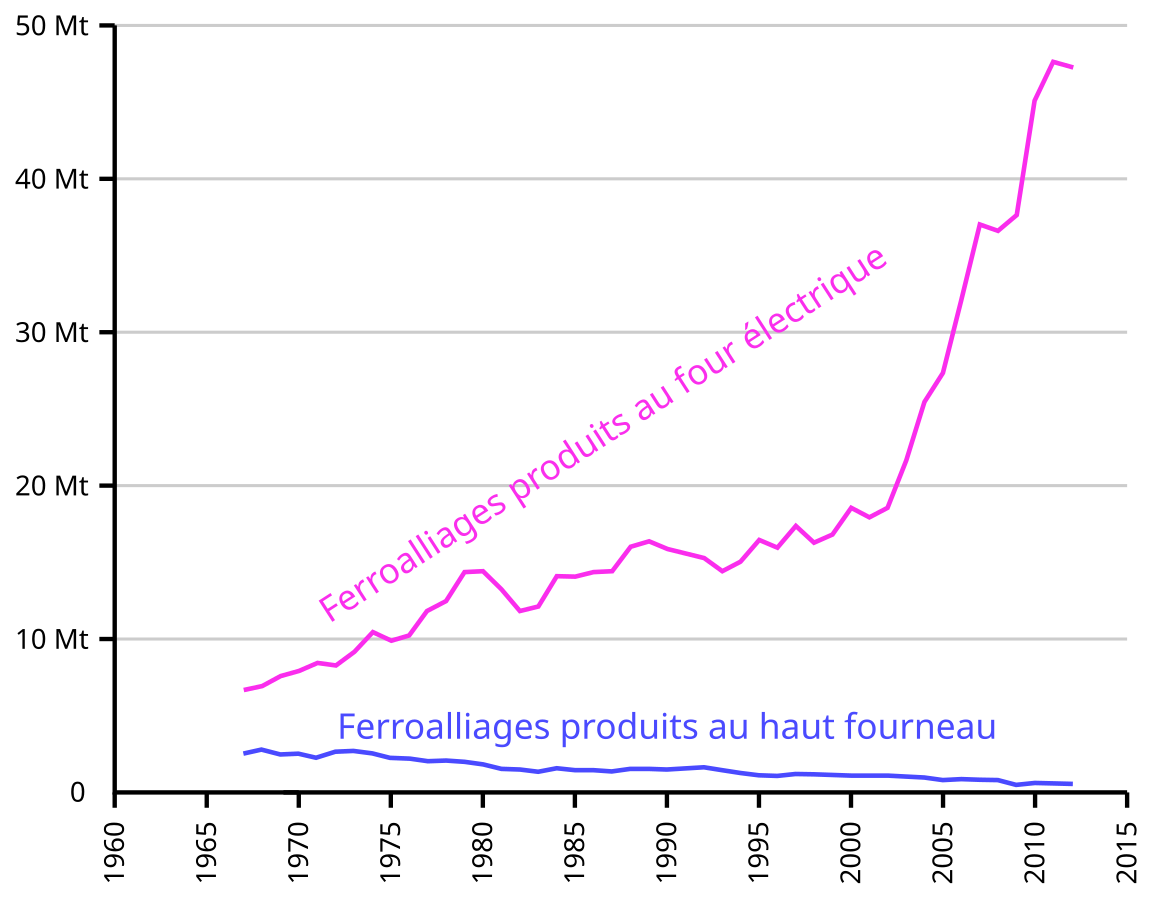
\includegraphics[width=\textwidth]{figures/Fig03}
%\end{minipage}\begin{minipage}{0.48\textwidth}
%\captionof{figure}{\'{E}volution de la production d'alliages de fer depuis 1960}
%\label{fig:01-03}

%\href{https://youtu.be/HWHX1vi-Vmc?si=za9wm9_b-DPp7t6T}{Principe de fonctionnement}
%\end{minipage}

%Le four électrique est très utilisé pour la synthèse de ferroalliages (chrome, manganèse, silicium, carbures) ou de métaux non ferreux : manganèse, plomb.


\section{Diagrammes d'Ellingham}

\subsection{Définition}

\definition{On cherche  étudier des réactions d'oxydo-réductions par voie sèche pour des couples \ce{Ox}/\ce{Red} dont l'équilibre rédox s'écrit : 
\begin{align*}
\ce{Red + O2(g) = Ox}
\end{align*}

On regardera l'évolution de l'enthalpie libre standard de réaction dans le cadre de l'hypothèse d'Ellingham où on considère que le couple $(\Delta_rH^\circ, \Delta_r S^\circ)$ est indépendant de la température. Ceci revient à dire que $\Delta_r C_p^\circ = 0$. Cette approximtion est légitime pour des études sur des plages modérées de température.

~ \

\faWarning ~ On regardera des réactions d'oxydo-réduction sèche pour une st{\oe}chiométrie en dioxygène de $-1$ ou $-1/2$ à préciser sur les diagrammes.
}

\subsection{Propriétés}

\subsubsection{\'{E}quation des droites d'Ellingham}
\definition{
Dans l'approximation d'Ellingham, l'enthalpie libre standard de réaction évolue de manière linéaire à condition qu'il n'y ait pas de changement d'état. En effet, l'équation s'écrit sous la forme : 
\begin{align*}
\Delta_r G^\circ = \underbrace{\Delta_r H^\circ}_{\text{ordonnée à l'origine}} \underbrace{- \Delta_r S^\circ}_{\text{pente}} T
\end{align*}}

\subsubsection{Signe de la pente}
\definition{
Dans le cas des couples d'oxyde de la forme \ce{MOy(s)}/\ce{MOx(s)}, toute équation rédox s'écrira sous la forme : 
\begin{align*}
\ce{MO_x(s) + O2(g) = MO_y (s)} \text{ avec } x < y
\end{align*}

Dans le cas de toute les transformation rédox, l'entropie standard de réaction est négative (c.-à-d. que l'état produit est plus organisé que l'état réactif) :
\begin{align*}
\Delta_r S^\circ < 0 \iff \text{pente} > 0
\end{align*}
}

Une exception importante est le carbone qui explique que le carbone constitue un réducteur universel des oxydes métalliques. Sachant que le carbone inorganique peut exister sous 3 degrés d'oxydation : 
\begin{center}
\begin{minipage}{0.58\textwidth}
\centering
\begin{tabular}{ccc}
\toprule
Degré d'oxydation & Forme chimique & Nom\\
\midrule
$0$ & \ce{C(s)} & Coke, charbon$\ldots$ \\
$+II$ & \ce{CO(g)} & Monoxyde de carbone \\
$+IV$ & \ce{CO2(g)} & Dioxyde de carbone \\
\bottomrule
\end{tabular}
\end{minipage}\begin{minipage}{0.38\textwidth}
\captionof{table}{Degrés d'oxydation du carbone inorganique}
\end{minipage}
\end{center}

On peut alors écrire trois couples rédox pour le carbone : 
\begin{center}
\begin{tabular}{cccc}
\toprule
Couples & \'{E}quation de réaction & Entropie standard de réaction $\Delta_r S^\circ$ & pente \\
\midrule
\ce{CO(g)}/\ce{C(s)} & \ce{2C(s) + O2(g) = 2CO(g)} & $>0$ & $<0$\\
\ce{CO2(g)}/\ce{C(s)} & \ce{C(s) + O2(g) = CO2(g)} & $\sim 0$ & $\sim 0$\\
\ce{CO2(g)}/\ce{CO(g)} & \ce{2CO(g) + O2(g) = 2CO2(g)} & $<0$ & $>0$\\
\bottomrule
\end{tabular}
\end{center}

On trouve alors trois tendances pour les trois couples d'Ellingham :
\begin{center}
\begin{minipage}{0.48\textwidth}
\centering
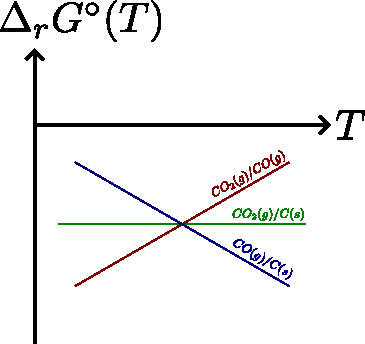
\includegraphics[width=0.8\textwidth]{figures/Fig09.pdf}
\end{minipage}\begin{minipage}{0.48\textwidth}
\captionof{figure}{Trois tendances différentes pour les couples du carbone inorganique}
\end{minipage}
\end{center}


\subsubsection{Ruptures de pente}
\definition{
En cas de changement d'état, la courbe d'Ellingham présente une rupture de pente à la température de transition à \SI{1}{\bar}.

\begin{center}
\begin{minipage}{0.48\textwidth}
\centering
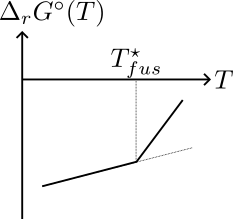
\includegraphics[width=0.5\textwidth]{figures/Fig04}
\end{minipage}\begin{minipage}{0.48\textwidth}
\captionof{figure}{Rupture de pente consécutive à une fusion}
\end{minipage}
\end{center}}

Par exemple, pour les couples \ce{ZnO(s)/Zn(s)} et \ce{ZnO(l)/Zn(s)}, une rupture de pente a lieu à \SI{693}{\kelvin}. Cela s'explique par le fait que l'état liquide a une entropie molaire plus grande que l'état solide. Ce gain s'entropie de réaction est dû à l'enthalpie de fusion de l'oxyde de zinc pur : 
\begin{align*}
\ce{2 Zn(s) + O2(g)  &= 2 ZnO(s)} ~ \times 1 \quad \Delta_r S^\circ (\ce{ZnO(s)}) \\
\ce{ZnO(s) &= ZnO(l)} ~ \times 2 \quad \Delta_{fus} S^\circ (\ce{ZnO(s)}) = \frac{\Delta_{fus} H^\circ (\ce{ZnO(s)})}{T_{fus}^\star} \\
\ce{2 Zn(s) + O2(g)  &= 2 ZnO(l)} ~ \times 1 \quad \Delta_r S^\circ (\ce{ZnO(l)})
\end{align*}

On en tire à partir de ces trois équilibres que : 
\begin{align*}
\Delta_r S^\circ (\ce{ZnO(l)}) = \Delta_r S^\circ (\ce{ZnO(s)}) + 2 \frac{\Delta_{fus} H^\circ (\ce{ZnO(s)})}{T_{fus}^\star}
\end{align*}


\subsubsection{Domaine de stabilité}
\paragraph{$\ldots$ dans un système isotherme}

~\

\definition{Le domaine de stabilité de l'oxydant (resp. le réducteur) du couple se trouve au-dessus (resp. en-dessous) de la courbe d'Ellingham.

\begin{center}
\begin{minipage}{0.48\textwidth}
\centering
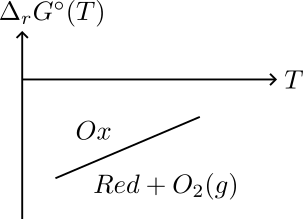
\includegraphics[width=0.5\textwidth]{figures/Fig05}
\end{minipage}\begin{minipage}{0.48\textwidth}
\captionof{figure}{Domaine de stabilité d'un couple \ce{Ox}/\ce{Red} dans le diagramme d'Ellingham}
\end{minipage}
\end{center}
}

Pour placer les domaines de stabilité, il faut donner un sens à l'axe des ordonnées. Revenons à l'équation de réaction modèle :
\begin{align*}
\ce{MO_x (s) + O2(g) = MO_y(s)} \quad x < y
\end{align*}

Cette réaction a pour enthalpie libre de réaction :
\begin{align*}
\Delta_r G = \mu^\star_{\ce{MOy}} - \left( \mu^\star_{\ce{MOx}} + \mu^\star_{\ce{O2}} \right)
\end{align*}

Par conséquent, si l'oxyde \ce{MO_y(s)} est plus stable que \ce{MO_x(s) + O2(g)}, on a alors : 
\begin{align*}
\mu^\star_{\ce{MOy}} < \left( \mu^\star_{\ce{MOx}} + \mu^\star_{\ce{O2}} \right) \iff \Delta_r G < 0
\end{align*}

Or, on sait exprimer l'enthalpie libre de réaction : 
\begin{align*}
\Delta_r G &= \Delta_r G^\circ  + RT \ln Q_r \\
&= \Delta_r G^\circ  + RT \ln \frac{P^\circ}{P_{\ce{O2}}} \text{ car }a(\ce{MO_x}) = 1
\end{align*}

Donc, on en tire que :
\begin{align*}
\Delta_r G^\circ < RT \ln \frac{P_{\ce{O2}}}{P^\circ} \iff RT \ln \frac{P_{\ce{O2}}^{eq}}{P^\circ} < RT \ln \frac{P_{\ce{O2}}}{P^\circ}
\end{align*}
puisque la constante de réaction équivaut à la valeur du quotient réactionnel à l'équilibre.

\definition{L'axe des ordonnées représente $RT \ln \frac{P_{\ce{P2}}}{P^\circ}$. Par conséquent, plus on monte sur l'axe des ordonnées, plus la pression en dioxygène est élevée.
\begin{center}
\begin{minipage}{0.48\textwidth}
\centering
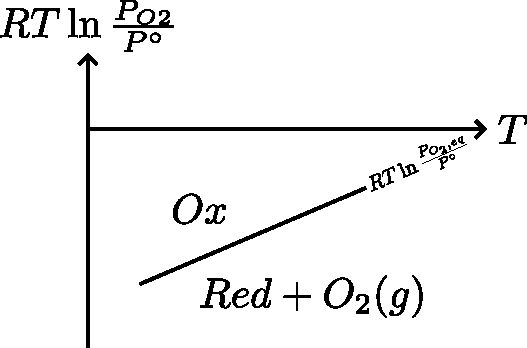
\includegraphics[width=0.8\textwidth]{figures/Fig10}
\end{minipage}\begin{minipage}{0.48\textwidth}
\captionof{figure}{Diagramme d'Ellingham : évolution de la "pression d'équilibre" en fonction de la température}
\end{minipage}
\end{center}
On en tire que pour une température donnée :
\begin{align*}
P_{O_2} > P_{O_2}^{eq}(T) &\iff \text{l'espèce oxydée est stable} \\
P_{O_2} = P_{O_2}^{eq}(T) &\iff \text{les espèces oxydée et réduite sont stables, donc coexistent} \\
P_{O_2} < P_{O_2}^{eq}(T) &\iff \text{l'expèce réduite est stable}
\end{align*}

\begin{center}
\begin{minipage}{0.48\textwidth}
\centering
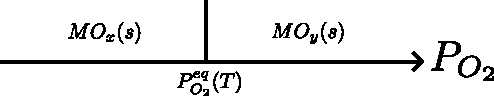
\includegraphics[width=0.8\textwidth]{figures/Fig10b}
\end{minipage}\begin{minipage}{0.48\textwidth}
\captionof{figure}{Stabilité du couple Ox/Red  \ce{MO_y}/\ce{MO_x} à une température $T$ donnée}
\end{minipage}
\end{center}

}


\paragraph{$\ldots$ dans un système à pression contrôlée}

~\
\definition{Lors d'une chauffe dans un four à pression contrôlée, il est possible en général de moduler la température d'inversion associée à l'oxydation en jouant sur la pression partielle en dioxygène : 
\begin{center}
\begin{minipage}{0.48\textwidth}
\centering
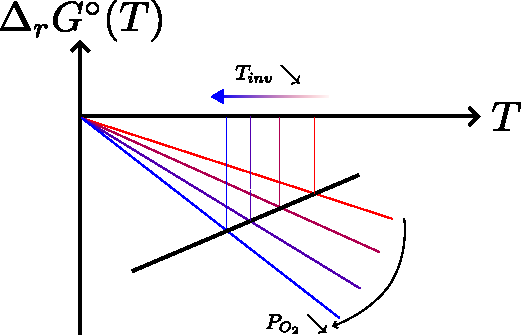
\includegraphics[width=0.8\textwidth]{figures/Fig11a}
\end{minipage}\begin{minipage}{0.48\textwidth}
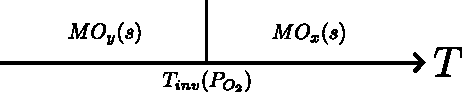
\includegraphics[width=\textwidth]{figures/Fig11b}
\captionof{figure}{Diagramme d'Ellingham : évolution de la température d'inversion en fonction de la pression partielle en dioxygène. Une diminution de la pression en dioxygène déplace la température d'inversion en augmentant le domaine de la stabilité de l'espèce réduite.}
\end{minipage}
\end{center}
}

En modulant la pression en dioxygène du système, on modifie le quotient réactionnel de la réaction 

\begin{align*}
\ce{MO_x (s) + O2(g) = MO_y (s)}
\end{align*}

Par conséquent, on cherche le nouvel équilibre tel que :

\begin{align*}
\Delta_r G \stackrel{eq}{=} 0 \iff \Delta_r G^\circ (T) -  RT \ln \frac{P_{O_2}}{P^\circ} = 0
\end{align*}

Pour trouver l'état d'équilibre, on doit trouver l'intersection entre la droite d'Ellingham $T \mapsto \Delta_r G^\circ (T)$ et la droite $T \mapsto R \ln\frac{P_{O_2}}{P^\circ} \cdot T$. La seconde droite est linéaire et a pour pente $R \ln \frac{P_{O_2}}{P^\circ}$


\section{Utilisation des diagrammes d'Ellingham}
\subsection{Element réducteur : le carbone}

\exercice{Element réducteur}{
Carbone = 2 couples rédox $\ce{CO(g)}$/$\ce{C(s)}$ et $\ce{CO2(g)}/\ce{CO(g)}$ 
\begin{align*}
\ce{C(s) + \frac{1}{2} O2(g) &= CO(g)} \\
\ce{CO(g) + \frac{1}{2} O2(g) &= CO2(g)} 
\end{align*}

\begin{center}
\begin{minipage}{0.58\textwidth}
\centering
\begin{tabular}{ccccc}
\toprule
Molécules & \ce{C(s)} & \ce{CO(g)} & \ce{CO2(g)} & \ce{O2(g)} \\
\midrule
$\Delta_f H^\circ ~ [\si{\kilo\joule\per\mole}]$ & $-$ & $-110.5$ & $-393.3$ & $0$\\
$S_m^\circ ~ [\si{\joule\per\mole\per\kelvin}]$ & $5.9$ & $197.9$ & $213.8$ & $205$\\
\bottomrule
\end{tabular}
\end{minipage}\hfill\begin{minipage}{0.38\textwidth}
\captionof{table}{Données thermodynamiques d'enthalpie de formation et d'entropies molaires à \SI{298}{\kelvin} [\href{https://www.wiredchemist.com/chemistry/data}{WiredChemist}]}
\end{minipage}
\end{center}

On choisira une stoechiométrie de $\frac{1}{2}$ pour \ce{O2}.

\Q Rappeler en quoi consiste l'approximation d'Ellingham.

\Q Tracer les droites d'Ellingham associées aux deux couples rédox.

\Q Calculer la température de dismutation de ce système. Que se passe-t-il au-dessus de la température d'inversion ? Proposer un nouveau couple rédox décrivant ce système et tracer sa droite d'Ellingham.}


\subsection{Element oxydant $\ldots$}
%\subsubsection{$\ldots$ les oxydes de cuivre}
\subsubsection{$\ldots$ les oxydes de fer}

Les oxydes de fer que l'on rencontre dans la nature sont la magnétite \ce{Fe3O4(s)}, l'oxyde ferrique \ce{Fe2O3(s)} et/ou l'oxyde ferreux \ce{FeO(s)}. 

\begin{center}
\begin{minipage}{0.68\textwidth}

\includegraphics[width=\textwidth]{figures/Fe-C-O.pdf}
\end{minipage}\hfill\begin{minipage}{0.28\textwidth}
\captionof{figure}{Diagramme d'Ellingham d'un système \ce{Fe-C-O} pour les espèces du fer et du carbone, pour une st{\oe}chiométrie en dioxygène de $-1$.}%Superposition du diagramme de Chaudron et de l'équilibre de Boudouard
\end{minipage}
\end{center}

D'après le diagramme d'Ellingham, on peut espérer réduire un mélange d'oxydes de fer (II,III) pour une température de four supérieure à \SI{1080}{\kelvin}.

\subsubsection{$\ldots$ les oxydes de silicium}

\exercice{Réduction du silicium}{
On se propose d'expliquer les conditions choisies industriellement pour la production du silicium. Celle-ci met en {\oe}uvre la réduction de la silice par le carbone, dans un four électrique à arc, à une température de l'ordre de \SI{1700}{\celsius}. La difficulté principale tient à ce que l'on doit éviter la formation de carbure \ce{SiC}, ce qui conduit à traiter dans le four un mélange dosé de sable (\ce{SiO2}) et de coke (carbone).

\textbf{Données :}  $T_{fus}^\star (\ce{Si}) = 1410 ~ \si{\celsius}$ ; $T_{vap}^\star (\ce{Si}) = 2355 ~ \si{\celsius}$.

\Q Considérant le diagramme d'Ellingham du silicium et du carbone, représenté sur la figure 1, justifier le choix du carbone comme réducteur. Trouver le domaine de température utilisable.

\Q Expliquer simplement pourquoi les segments (1) et (2) d'une part, (3) d'autre part ont des pentes de signe contraire. 

Interpréter physiquement le changement de pente au point \textbf{A}.


Sachant que l'augmentation de la pente est voisine de \SI{30}{\joule\per\mole\per\kelvin}, en déduire une estimation de la variation d'enthalpie $\Delta_t H^\circ (\ce{Si})$ de la transformation mise en jeu. Sous quelle forme physique récupère-t-on le silicium produit par ce procédé ?

\begin{center}
\begin{minipage}{0.48\textwidth}
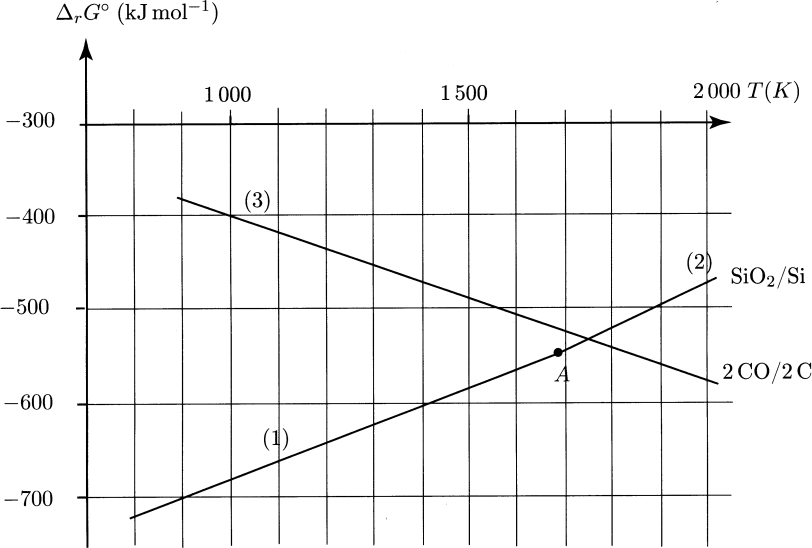
\includegraphics[width=\textwidth]{figures/Fig07}
\end{minipage}\hfill\begin{minipage}{0.48\textwidth}
\captionof{figure}{Diagramme d'Ellingham des couples \ce{SiO2}/\ce{Si} et \ce{2CO/2C}, soit pour une st{\oe}chiométrie en dioxygène de $-1$.}
\end{minipage}
\end{center}

Les équations des segments (2) et (3) sont respectivement :
\begin{align*}
\Delta_r G^\circ_2 (T) &= -907 \cdot 10^3 + 213 \cdot T \quad [\si{\joule\per\mole}] \\
\Delta_r G^\circ_3 (T) &= -221 \cdot 10^3 - 179 \cdot T \quad [\si{\joule\per\mole}\text{ de }\ce{O2}]
\end{align*}

Montrer que la réduction de la silice par le carbone est endothermique.

Pour obtenir les renseignements nécessaires à la métallurgie du silicium, nous allons utiliser les diagrammes de stabilité thermodynamique : ils permettent de déterminer les phases stables en présence d'une phase gazeuse. Nous choisissons comme réducteur gazeux le monoxyde de carbone, produit d'oxydation du carbone à haute température.

%Pour obtenir les renseignements nécessaires à la métallurgie du silicium, nous allons utiliser les diagrammes de stabilité thermodynamique : ils permettent de déterminer les phases stables en présence d'une phase gazeuse. 

\begin{center}
\begin{minipage}{0.48\textwidth}
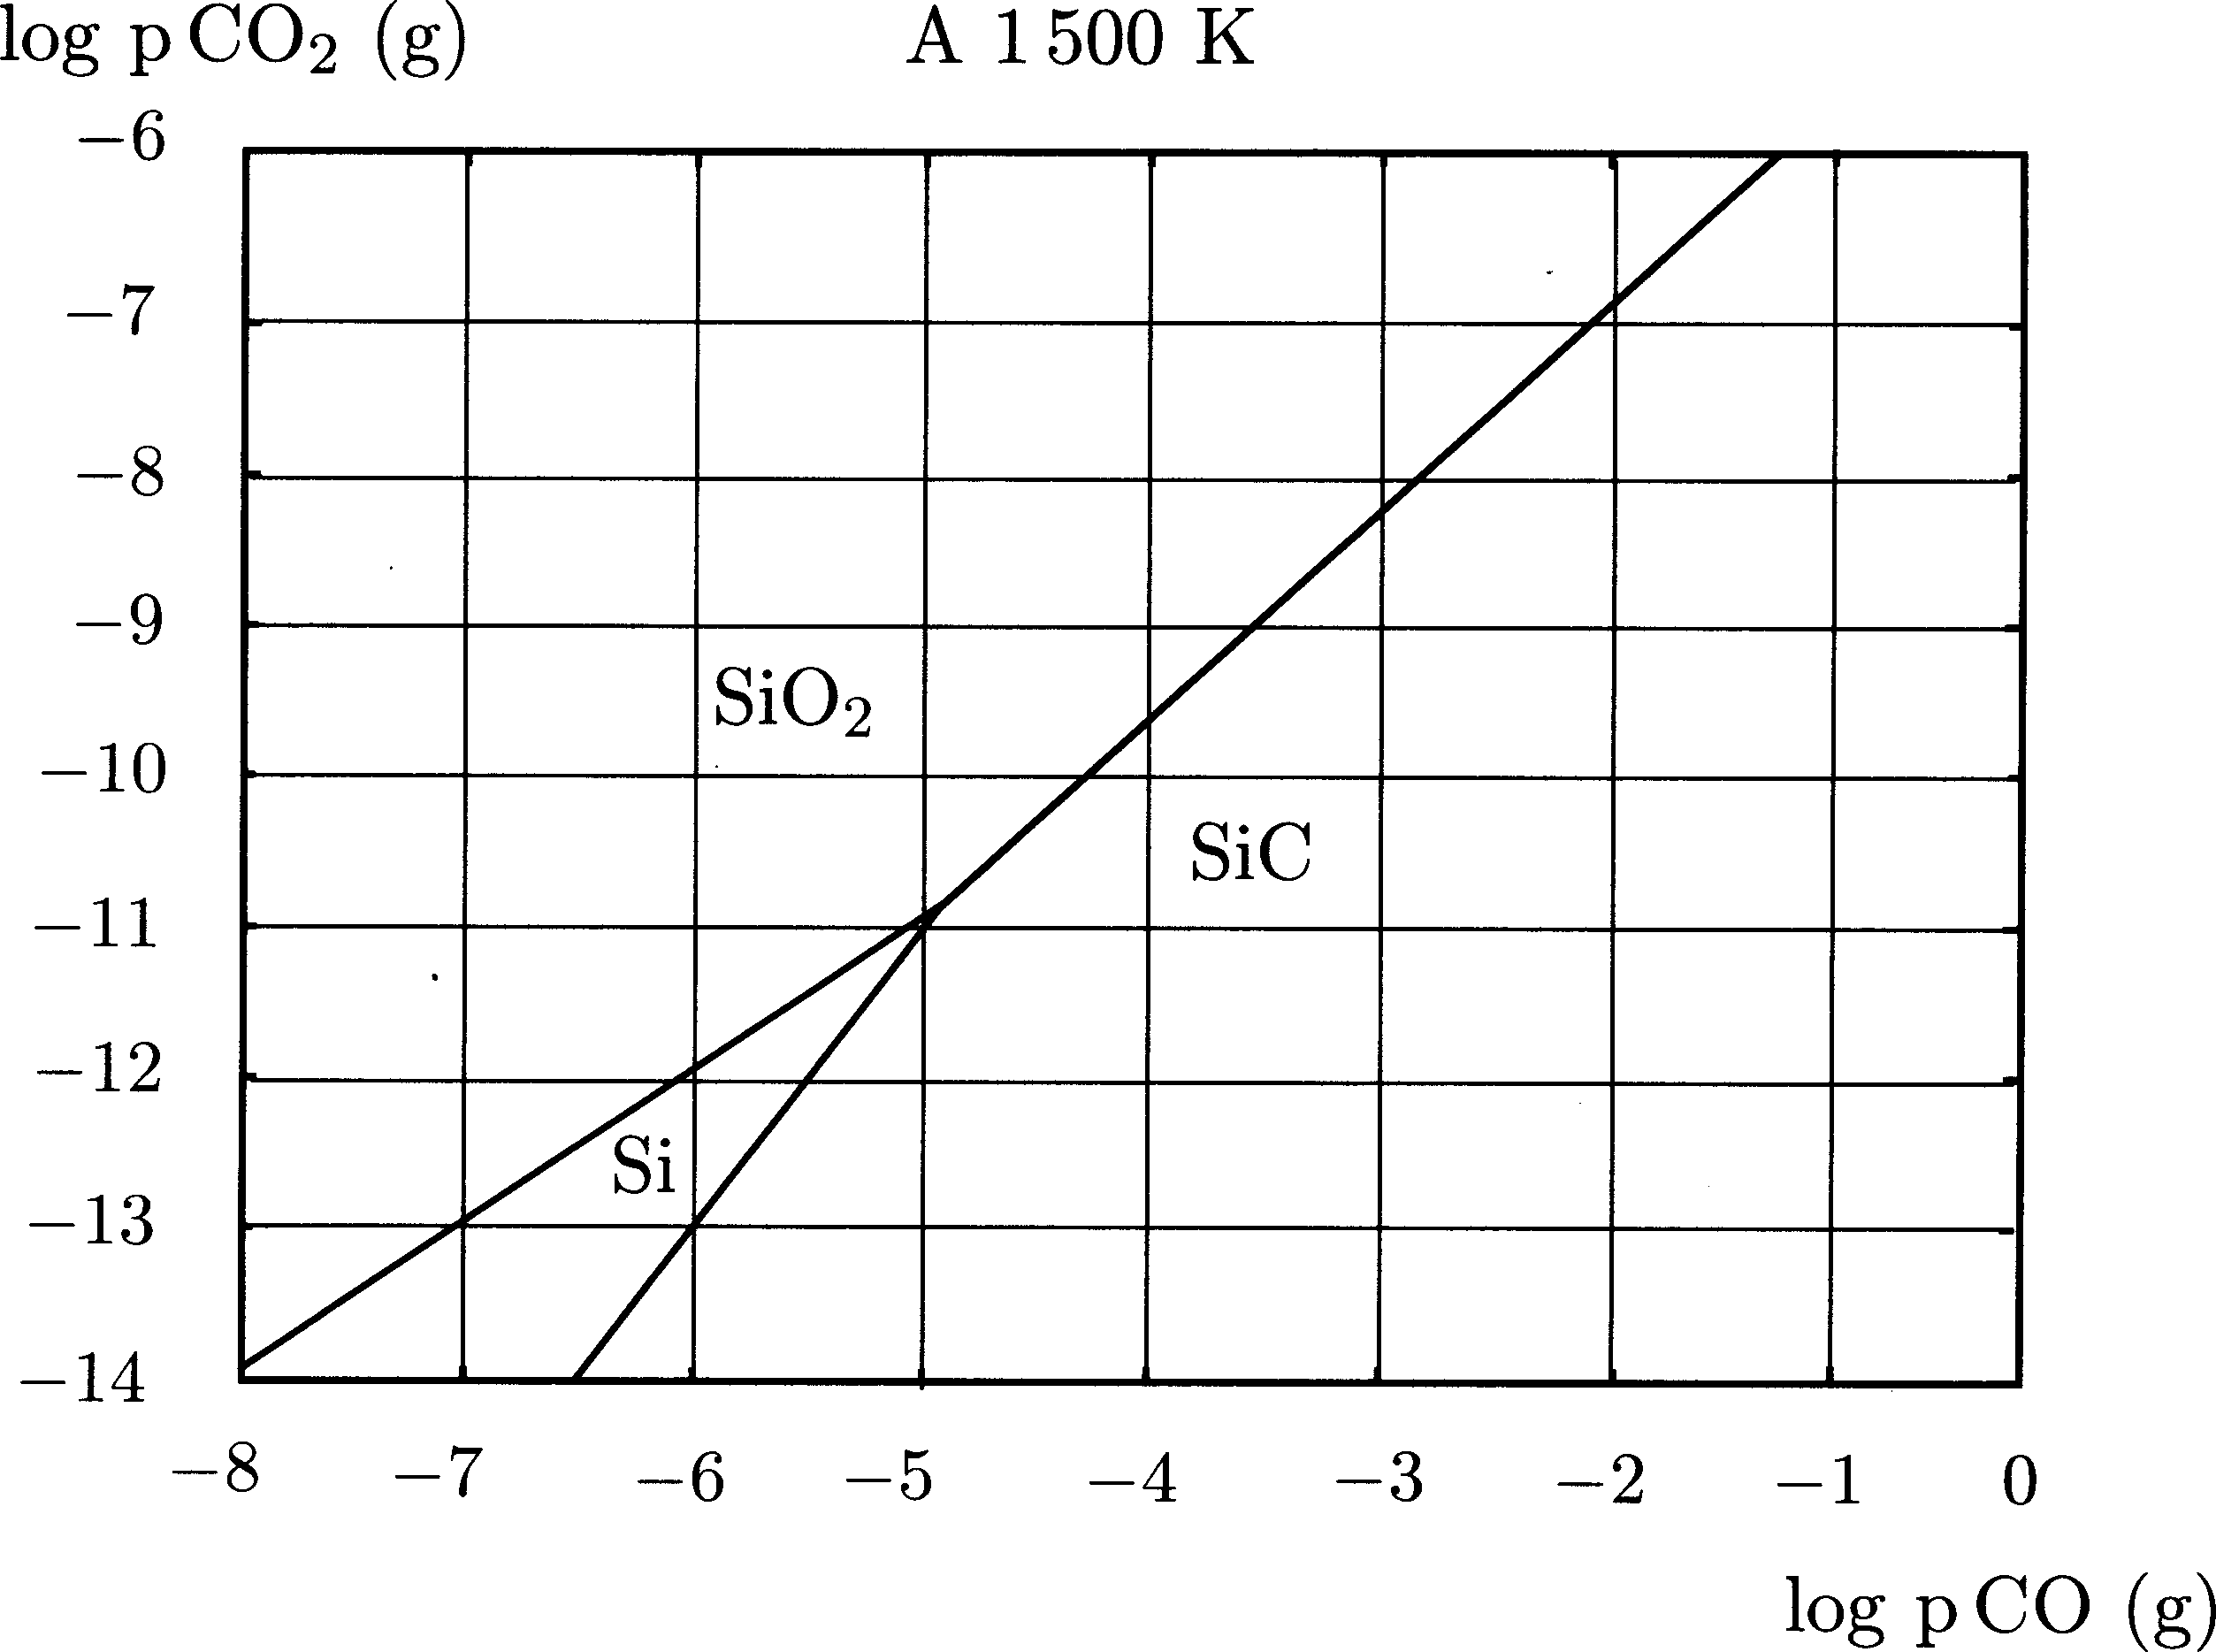
\includegraphics[width=\textwidth]{figures/Fig06}
\end{minipage}\hfill\begin{minipage}{0.48\textwidth}
\captionof{figure}{Diagramme de stabilité thermodynamique du système \ce{Si-C-O} à \SI{1500}{\kelvin}}
\end{minipage}
\end{center}

Les solides envisagés sont \ce{Si}, \ce{SiO2} et \ce{SiC} en présence d'une phase gazeuse contenant \ce{CO(g) + CO2(g)}.

\Q Déterminer les pentes des trois segments connaissant les coordonnées du point triple à \SI{1500}{\kelvin} ($\log p(\ce{CO}) = -4.9$ et $\log p(\ce{CO2}) = -10.8$) et les coordonnées de trois autres points :

\begin{center}
\begin{minipage}{0.48\textwidth}
\begin{tabular}{cccc}
\toprule
Couple à \SI{1500}{\kelvin} & \ce{SiO2}/\ce{Si} & \ce{SiO2}/\ce{SiC} & \ce{SiC}/\ce{Si} \\
\midrule
$\log p(\ce{CO})$ & $-8.0$ &  $-2.0$ & $-6.5$ \\
$\log p(\ce{CO2})$ & $-13.9$ & $-6.9$ &  $-14.0$ \\
\bottomrule
\end{tabular}
\end{minipage}\hfill\begin{minipage}{0.48\textwidth}
\captionof{table}{Point de trois courbes d'Ellingham différentes à \SI{1500}{\kelvin}}
\end{minipage}
\end{center}


En déduire les équations des équilibres chimiques correspondant aux trois frontières.

\Q Quelle est la valeur de la variance du système au point triple ? Justifier.

\Q Donner une valeur approchée de la constante d'équilibre relative à la réduction de la
silice en silicium par le monoxyde de carbone à 1500 K.

\Q Déduire des données précédentes les raisons d'une limitation impérative de la quantité
de carbone dans le procédé industriel d'élaboration du silicium.
}

%https://microelectronique.univ-rennes1.fr/fr/index_chap3.htm
Cette première étape au four à arc électrique est suivie d'un procédé de purification par distillation. Pour cela, on forme le trichlorosilane \ce{SiHCl3} par réaction du silicium avec l'acide chlorhydrique : 
\begin{align*}
\ce{Si(s) + 3HCl (g) ->[300 \si{\celsius}] SiHCl3(g) + H2(g)}
\end{align*}

Cette espèce fortement volatile ($T_{eb}^\star (1 ~ \si{\bar}) \approx 31 ~ \si{\celsius}$) est distillable et peut-être re-réduite en silicium de haute pureté : 
\begin{align*}
\ce{SiHCl3(g) + H2(g) -> Si(s) + 3HCl(g)}
\end{align*}
Ce silicium se dépose, et à partir d'un germe, cristallise sous la forme d'un lingot polycristallin de haute pureté. On atteind des puretés de l'ordre du ppm.


Certaines applications nécessitent l'utilisation de silicium monocristallin. On l'obtient à partir de silicium polycristallin de haute pureté, utilisé comme charge dans un creuset en graphite et est fondue à haute température. On réalise alors un tirage, appelée tirage de Czochralski, en tirant un bras mécanique initialement plongé dans le creuset en graphite. Une animation est disponible au lien suivant : 
\begin{center}
\url{https://microelectronique.univ-rennes1.fr/animation/czochraslski/czochraslski2.gif}
\end{center}

Le diamètre du cristal est lié à la vitesse de tirage.



\end{document}
